\documentclass[aspectratio=169]{beamer}

\usetheme{dpb}

\setbeamertemplate{theorems}[numbered]

\usepackage[citestyle=numeric]{biblatex}
\addbibresource{../references.bib}

\usepackage{graphicx}

\usepackage{tikz}
\usetikzlibrary{
	overlay-beamer-styles,
	positioning,
	fit,
	arrows,
	petri,
	shapes.geometric,
	shapes.symbols
}

\usepackage{amsmath}
\usepackage{mathtools}

\newcommand{\source}[1]{\ensuremath{\text{source}\left[{#1}\right]}}
\newcommand{\dest}[1]{\ensuremath{\text{dest}\left[{#1}\right]}}
\newcommand{\isfinal}[1]{\ensuremath{\text{isFinal}\left({#1}\right)}}

\newtheorem{proposition}{Proposition}
\theoremstyle{definition}
\theoremstyle{remark}
\newtheorem{axiom}{Assumption}
\newtheorem{observation}{Observation}

\newcommand*{\vcenteredhbox}[1]{\begingroup
	\setbox0=\hbox{#1}\parbox{\wd0}{\box0}\endgroup}

\setlength{\parskip}{\baselineskip}


\title{A Change Data Capture System for SpazioDati}
\subtitle{Thesis Presentation}
\date{2021-03-15}
\institute{Università degli Studi di Trento}
\author{Daniele Parmeggiani}


\begin{document}

\pagenumbering{gobble}
\inserttitleframe
\pagenumbering{arabic}

\begin{frame}{Context and Scope}
	\begin{center}
	\begin{tabular}{cc}
		
\includegraphics[width=.45\linewidth]{spaziodati.png} \hspace*{1cm} & 
\includegraphics[width=.4\linewidth]{atoka.pdf}
	\end{tabular}
	\end{center}
\end{frame}

\begin{frame}{Change Data Capture Systems}
	\begin{figure}
		\centering
		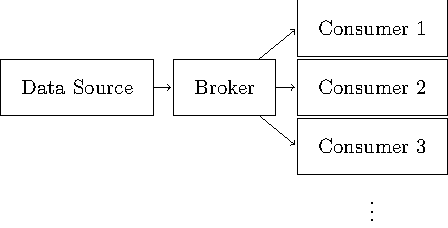
\includegraphics[width=0.7\linewidth]{../figures/introduction/cdc-generic}
	\end{figure}
\end{frame}

\begin{frame}{Proposed CDC System Design}
	\begin{center}
	\centering{\resizebox{1.35\textheight}{!}{
	\begin{tikzpicture}[
		node distance=5mm,
		shorten >=1pt,
		->
		]
		
		\node[draw, tape] (tables) {Table Data};
		\node[draw, right=of tables] (wal) {Write-Ahead Log};
		\path (tables) edge (wal);
		\node[above=of tables, yshift=-5mm] (p) {\phantom{PostgreSQL}};
		\begin{scope}
			\node[draw, cylinder, shape border rotate=90, aspect=0.1, fit=(tables)(wal)(p)] (postgres) {};
		\end{scope}
		\node[below=of postgres.north, yshift=-5pt] (po) {PostgreSQL};
		
		\node[draw, cloud, aspect=2, left=of postgres, visible on=<2->] (other) {Other Systems};
		\path (postgres) edge [pre, bend left, visible on=<2->] (other);
		\path (other) edge [pre, bend left, visible on=<2->] (postgres);
		
		\node[draw, right=of postgres, right=15mm, visible on=<3->] (debezium) {Debezium};
		\path (postgres) edge[visible on=<3->] (debezium);
		
		\node[draw, below=of debezium, below=15mm, visible on=<3->] (kafka) {
			\small\begin{tabular}{c}
				{\normalsize Kafka} \\
				\emph{per-table topics}\\
				\begin{tabular}{cccc}
					$\alpha$&$\beta$&$\gamma$&$\delta$\\
					$\epsilon$&$\zeta$&$\eta$&$\theta$\\
					$\iota$&$\kappa$&$\lambda$&\\
				\end{tabular}
			\end{tabular}
		};
		\path (debezium) edge[visible on=<3->] (kafka);
		
		\node[draw, below left=of kafka, visible on=<4->] (streams) {
			\small\begin{tabular}{c}
				{\normalsize Kafka Streams} \\
				\emph{per-table streams}\\
				\begin{tabular}{cccc}
					$\eta$&$\theta$&$\kappa$&$\lambda$\\
				\end{tabular}
			\end{tabular}
		};
		\path (kafka) edge[visible on=<4->] (streams);
		
		\node[draw, above left=of streams, visible on=<4->] (connect) {
			\small\begin{tabular}{c}
				{\normalsize Kafka Connect} \\
				\emph{per-table connectors}\\
				\begin{tabular}{cccc}
					$\alpha$&$\beta$&$\gamma$&$\delta$\\
					$\epsilon$&$\zeta$&$\eta$&$\theta$\\
					$\iota$&$\kappa$&$\lambda$&\\
				\end{tabular}
			\end{tabular}
		};
		\path (kafka) edge[visible on=<4->] node[auto,swap, visible on=<4->] {\small{except $\eta$, $\theta$, $\kappa$, $\lambda$}} (connect);
		\path (streams) edge[visible on=<4->] (connect);
		
		\node[draw, cylinder, shape border rotate=90, aspect=0.1, left=of connect, visible on=<4->] (output) {Output Database};
		\path (connect) edge[visible on=<4->] (output);
		
		\begin{scope}
			\node[draw, dashed, fit=(postgres), label=above:{Data Source}] (ds) {};
		\end{scope}
		\begin{scope}
			\node[draw, dashed, fit=(debezium)(kafka), label=above:{\only<3->{Broker}}, visible on=<3->] (broker) {};
		\end{scope}
		\begin{scope}
			\node[draw, dashed, fit=(streams)(connect)(output), label=below:{\only<4->{Consumers}}, visible on=<4->] (consumers) {};
		\end{scope}
		
	\end{tikzpicture}
	}}
	\end{center}
\end{frame}

\begin{frame}{Duality of Tables and Streams}
	\begin{center}
	\centering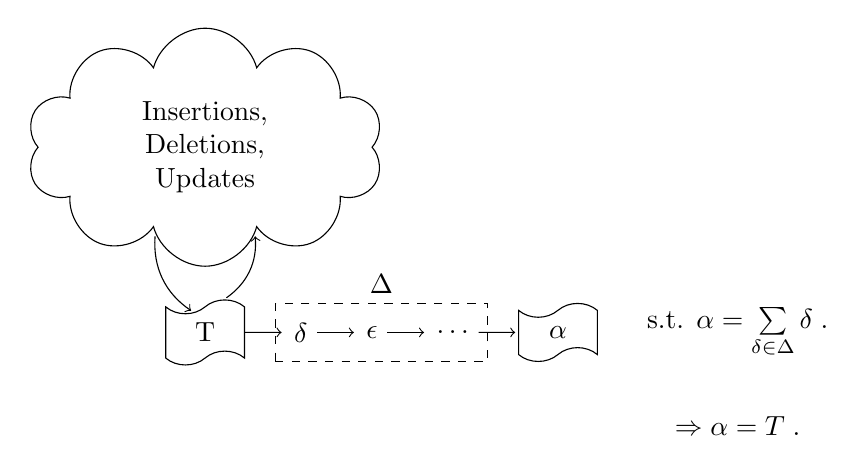
\begin{tikzpicture}[
		node distance=5mm,
		shorten >=1pt,
		->
		]
		
		\node[draw, tape, minimum width=10mm] (T) {T};
		\node[draw, cloud, aspect=2, above=of T] (other) {
			\begin{tabular}{c}
				Insertions, \\ Deletions, \\ Updates
			\end{tabular}
		};
		\path (T) edge [pre, bend left] (other);
		\path (other) edge [pre, bend left] (T);
		
		\node[right=of T] (d) {$\delta$};
		\node[right=of d] (e) {$\epsilon$};
		\node[right=of e] (ell) {$\ldots$};
		\path (T) edge (d);
		\path (d) edge (e);
		\path (e) edge (ell);
		\begin{scope}
			\node[draw, dashed, fit=(d)(e)(ell), label=above:{$\Delta$}] (D) {};
		\end{scope}
		
		\node[draw, tape, minimum width=10mm, right=of ell] (a) {$\alpha$};
		\path (ell) edge (a);
		\node[right=of a] (st) {
			s.t. $ \alpha = \sum\limits_{\delta \in \Delta} \delta \; . $
		};
		\node[below=of st] (modus-ponens) {$\Rightarrow \alpha = T \; .$};
		
	\end{tikzpicture}
	\end{center}
\end{frame}

\begin{frame}{Classes of Tables}
	\begin{itemize}
		\item Plain:
			$
			\dest{\omega} := \pi_S(\source{\omega})
			$
		\item Aggregated
		\item Time-traveled
	\end{itemize}
\end{frame}

\begin{frame}{Aggregated Tables}
	\begin{tabular}{ll}
		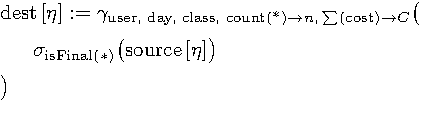
\includegraphics{agg-eta} & 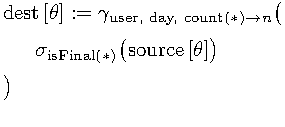
\includegraphics{agg-theta} \\
		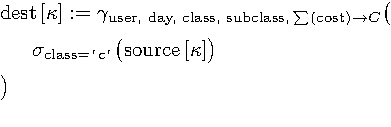
\includegraphics{agg-kappa} & 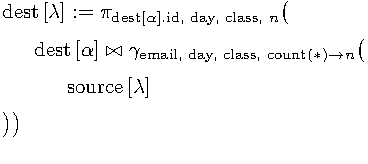
\includegraphics{agg-lambda}
	\end{tabular}
\end{frame}

\begin{frame}{Time Travel}
	\begin{figure}
		\centering
		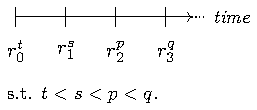
\includegraphics[width=0.4\linewidth]{../figures/time-travel/intro}
		\caption{Representation of changes to a row $r$.}
		\label{fig:tt-intro}
	\end{figure}

	Was part of official PostgreSQL distributions, up to version 12.
\end{frame}

\begin{frame}{Validity Column}
	\begin{table}
		\centering
		\begin{tabular}{cc}
			$r$ & \emph{validity} \\
			\hline
			$0$ & $[t, +\infty)$ \\
		\end{tabular}
		\hspace{1mm}
		\begin{tabular}{cc}
			$r$ & \emph{validity} \\
			\hline
			$0$ & $[t, s)$ \\
			$1$ & $[s, +\infty)$ \\
		\end{tabular}
		\hspace{1mm}
		\begin{tabular}{cc}
			$r$ & \emph{validity} \\
			\hline
			$0$ & $[t, s)$ \\
			$1$ & $[s, p)$ \\
			$2$ & $[p, +\infty)$ \\
		\end{tabular}
		\hspace{1mm}
		\begin{tabular}{cc}
			$r$ & \emph{validity} \\
			\hline
			$0$ & $[t, s)$ \\
			$1$ & $[s, p)$ \\
			$2$ & $[p, q)$ \\
			$3$ & $[q, +\infty)$ \\
		\end{tabular}
		\caption{Representation in $\dest{\omega}$ of the changes outlined in Figure \ref{fig:tt-intro}.}
		\label{tab:tt-validity}
	\end{table}
\end{frame}

\begin{frame}{Time Travel Mapping}
	\begin{equation}\label{tt:insert}
		\source{\omega} \rightarrow \text{\texttt{INSERT} } r_i^t \xRightarrow{\tau}
		\text{\texttt{INSERT} } r_i \text{ s.t. } \text{validity} := [t, +\infty)
	\end{equation}
	
	\begin{equation}\label{tt:update}
		\source{\omega} \rightarrow \text{\texttt{UPDATE} } r_i^t \xRightarrow{\tau}
		\begin{Bmatrix}
			\text{1. \texttt{UPDATE} } r_{i-1} \text{ s.t. } \text{validity} \cap (-\infty, t) \\
			\text{2. \texttt{INSERT} } r_i \text{ s.t. } \text{validity} := [t, +\infty)
		\end{Bmatrix}
	\end{equation}
	
	\begin{equation}\label{tt:delete}
		\source{\omega} \rightarrow \text{\texttt{DELETE} } r_i^t \xRightarrow{\tau}
		\text{\texttt{UPDATE} } r_{i-1} \text{ s.t. } \text{validity} \cap (-\infty, t)
	\end{equation}
\end{frame}

\begin{frame}{On Constraints}
	\begin{itemize}
		\item uniqueness (including primary-key),
		\item conditional (including non-null), and
		\item referential integrity (foreign-key).
	\end{itemize}
	\vspace{\parskip}
	\only<2->{\begin{axiom}
		$\source{*}$ is consistent.
	\end{axiom}}
\end{frame}

\begin{frame}{Foreign Key Constraints}
	\begin{figure}
		\centering
		\begin{tabular}{p{0.45\textwidth} p{0.45\textwidth}}
			\vspace{0pt} 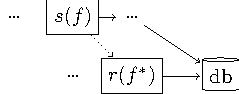
\includegraphics[width=0.4\textwidth]{../figures/data/fk-stream} &
			\vspace{0pt} \only<2->{ 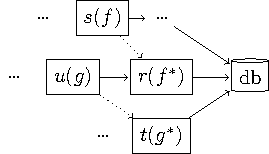
\includegraphics[width=0.44\textwidth]{../figures/data/fk-stream-recurrence}}
		\end{tabular}
	\end{figure}
\end{frame}

\end{document}
